
\section{Project Tango}

Project Tango ist eine Technologie Plattform für Android Tablets und Smartphones von Google’s Advanced Technology and Projects Group (ATAP). Das Ziel dieser Plattform ist es Motion Tracking (Positionierung), Depth Perception (Tiefeninformation/Pointcloud) und Area Learning (Lokalisierung) auf mobile Endgeräte zu bringen, um verschiedenste Anwendungs-Szenarien abzudecken. Typische Szenarien sind Indoor Navigation, Virtual Reality Anwendungen, Vermessungs- und Rekonstruktions Software und Augmented Reality Anwendungen.

Es ermöglicht in erster Linie ein Tracking von Positionsänderungen des Geräts im Raum und bietet somit eine genaue relative Lokalisierung. Mit Hilfe dieser Lokalisierung und der Hinzunahme von visuellen Merkmalen im Raum, ist das Gerät in der Lage, seine Umgebung kennenzulernen und gegebenenfalls die Lokalisierung zu korrigieren oder aber in einer bereits erlernten Umgebung zu ermitteln. Zusätzlich bietet Project Tango die Möglichkeit mit Hilfe eines Tiefensensors eine Pointcloud der Tiefeninformation pro Bildausschnitt zu liefern, um Anwendungen auch Räumliche Informationen bereitzustellen.  \citep{Proje19:online}

\subsection{Geräte und Hardware}

Da das Project Tango zum Zeitpunkt der Verfassung dieser Thesis noch unter Entwicklung steht, gibt es von Google die Entwickler Prototypen. Das Erste Gerät im Smartphone Format, welches in Abbildung \ref{fig:tango-device} rechts unten zu erkennen ist, wurde bereits durch eine neue Generation rechts oben ersetzt. Dieses 7\dq Tablet verfügt, wie in Abbildung \ref{fig:tango-device} links zu erkennen, über einen Infrarot Laser Projektor, eine Fisheye Camera und eine normale 4 Megapixel Kamera auf der Rückseite. Zudem sind, wie von aktuellen Smartphones bekannt, ein Beschleunigungssensor, Umgebungslichtsensor, Barometer, Kompass, GPS und ein Gyroskop verbaut. Das Gerät wird von einem NVIDIA Tegra K1 Prozessor betrieben und verfügt über 4GB Arbeitsspeicher. \citep{Proje19:online} Mit diesem Gerät wurden die später beschriebenen Techniken umgesetzt und evaluiert. 

\begin{figure}[h]
  \centering
	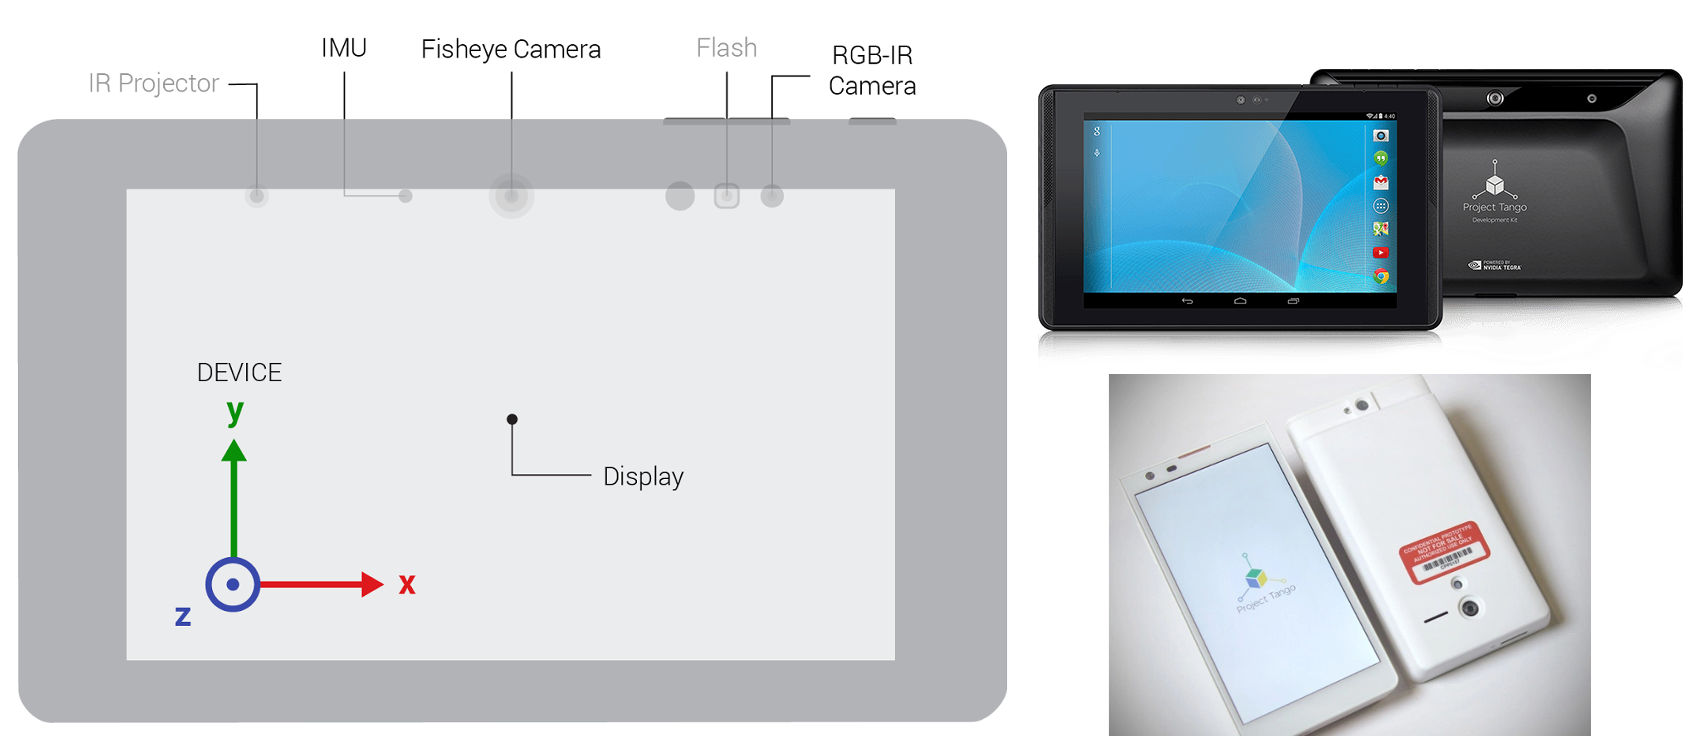
\includegraphics[width=1.0\textwidth]{content/images/theory/tango-device.png} 
  \caption{Links: schematischer Aufbau der Google Project Tango Hardware. Rechts: Das aktuelle Entwickler Gerät im Tablet Faktor (oben) und das alte Entwickler Gerät im Smartphone Faktor (unten). Übernommen von \citet{GoogleDevelopers:online}}
  \label{fig:tango-device}
\end{figure}

\subsection{Konzepte und Schnittstellen}

Generell betrachtet ist das Project Tango eine Plattform, die Computer Vision nutzt, um dem Gerät die Möglichkeit bietet seine relative Positionierung in der umgebenen Szene live zu bestimmen. Auf den Geräten kommt Googles Android zum Einsatz, weshalb zu beachten ist, dass es sich bei der Platform nur Bedingt um eine Echtzeit Umgebung handelt. Das liegt daran, dass der Linux Kernel keine Garantien für die zeitlich präzise Ausführung von Instruktionen  auf Grund von Scheduling geben kann. Google weist daher darauf hin, dass das System als \enquote{soft-realtime} betrachtet werden sollte. Daher sollten Messergebnisse verschiedener Sensoren unter Berücksichtigung ihrer Aufnahme Zeitstempel verwendet werden. \citet{GoogleDevelopersConcepts:online}

\subsubsection{Motion Tracking}

Um die relative Bewegung vom Start des Project Tango Systems bestimmen zu können nutzt es \enquote{visual-inertial odometry}. 

Visual Odometry von \citet{nister2004visual} ist in der Lage aus einfachen Video Inhalten in Echtzeit die Bewegung der Kamera zu bestimmen. Hierzu werden zunächst übergreifende Features über mehrere Bilder des Videos bestimmt, woraus mit Hilfe des 5-point Algorthmus von 

Motion tracking means that a Project Tango device can track its own movement and orientation through 3D space. Walk around with a device and move it forward, backward, up, down, or tilt it in any direction, and it can tell you where it is and which way it's facing. It's similar to how a mouse works, but instead of moving around on a flat surface, the world is your mousepad.

Project Tango implements motion tracking using visual-inertial odometry, or VIO, to estimate where a device is relative to where it started. Unlike GPS, motion tracking using VIO works indoors and can provide higher accuracy.

Standard visual odometry uses camera images to determine a change in position by looking at the relative position of different features in those images. For example, if you took a photo of a building from far away and then took another photo from closer up, it would be possible to calculate the distance the camera moved based on the change in size and position of the building in the photos.

Visual-inertial odometry supplements visual odometry with inertial motion sensors capable of tracking a device's rotation and acceleration. This allows a Project Tango device to estimate both its orientation and movement within a 3D space with even greater accuracy.

Motion tracking is great by itself if you need to know a device's orientation and relative position, but there are some limitations:

Over long distances and periods of time the accumulation of small errors can cause measurements to "drift," leading to larger errors in absolute position.
Motion tracking does not understand the actual area around it. Every time you start a new motion tracking session, the tracking starts over and reports its position relative to its most recent starting position.
Both of these limitations are addressed by the next core technology, area learning.

For information on how to write applications using motion tracking, see the developer overview on Motion Tracking.

\subsubsection{Deph Perception}

\subsubsection{Area Learning}


\subsection{Einordnung zu Augmented Reality}

Um das Project Tango in den zuvor erwähnten technologischen Charakteristika einordnen zu können, wird zunächst einmal auf die technischen Details der Plattform eingegangen. 
